\documentclass[11pt]{article}

\usepackage{fullpage}
\usepackage{graphicx}
\usepackage{amsmath}
\usepackage{amssymb}
\usepackage{amsthm}
\usepackage{fancyvrb}
% \usepackage{algorithm}
\usepackage{wrapfig}
% \usepackage[noend]{algpseudocode}
\usepackage{xcolor}
\usepackage{tcolorbox}
\usepackage{tikz}
\usepackage{float}
\usepackage{hyperref}
\tcbuselibrary{theorems, breakable}

\theoremstyle{definition}
\newtheorem{definition}{Definition}
\theoremstyle{plain}
\newtheorem{theorem}{Theorem}
\newtheorem{lemma}{Lemma}
\newtheorem{corollary}{Corollary}
\theoremstyle{remark}
\newtheorem{remark}{Remark}
\newtheorem{example}{Example}

\parindent0in
\pagestyle{plain}
\thispagestyle{plain}
\graphicspath{{./}}

%% UPDATE MACRO DEFINITIONS %%
\newcommand{\myname}{Scribed By: Anupam Dwivedi (2025201032)}
\newcommand{\mynami}{Name 2 (Roll No. 2)}

\newcommand{\assignment}{Lecture \#Num}
\newcommand{\duedate}{$2^{nd}$ Apr 2026}
\newtheorem*{thmtype}{Outline}
\newcommand{\statement}{
This lecture covers the foundational theory of constrained optimization. We study feasible and descent directions, characterize local minima via the interaction of these direction sets, introduce active constraints, and build toward a matrix-form necessary condition. We conclude with Farkas' Lemma and its corollary, which provides the algebraic machinery underlying the KKT conditions.
}

\begin{document}

\textbf{IIIT Hyderabad}\hfill\textbf{\myname}\\[0.01in]
\textbf{-}\hfill\textbf{\mynami}\\[0.01in]
\textbf{Optimization Methods (CS1.404)}\hfill\textbf{\assignment}\\[0.01in]
\textbf{Instructor: Dr.\ Naresh Manwani}\hfill\textbf{\duedate}\\
\smallskip\hrule\bigskip

\begin{thmtype}
\statement
\end{thmtype}

% =====================================================================
\section{Feasible and Descent Directions in Constrained Optimization}
% =====================================================================

We consider the general constrained optimization problem:
\begin{equation}
  \min_{x \in \mathbb{R}^n} \; f(x) \quad \text{subject to} \quad g_i(x) \leq 0, \quad i = 1, \ldots, m,
  \label{eq:prob}
\end{equation}
where $f, g_i : \mathbb{R}^n \to \mathbb{R}$ are continuously differentiable. The \emph{feasible set} is
\[
  \mathcal{X} = \{x \in \mathbb{R}^n : g_i(x) \leq 0, \; i = 1, \ldots, m\}.
\]

\begin{definition}[Feasible Direction]
  A nonzero vector $d \in \mathbb{R}^n$ is called a \textbf{feasible direction} at a point $x \in \mathcal{X}$ if there exists $\bar{\alpha} > 0$ such that
  \[
    x + \alpha d \in \mathcal{X} \quad \text{for all } \alpha \in (0, \bar{\alpha}).
  \]
  Intuitively, $d$ points \emph{into} the feasible set from $x$; moving a small step along $d$ keeps us feasible.
\end{definition}

\begin{definition}[Descent Direction]
  A nonzero vector $d \in \mathbb{R}^n$ is called a \textbf{descent direction} for $f$ at $x$ if there exists $\bar{\alpha} > 0$ such that
  \[
    f(x + \alpha d) < f(x) \quad \text{for all } \alpha \in (0, \bar{\alpha}).
  \]
  That is, moving along $d$ from $x$ strictly decreases the objective.
\end{definition}

\textbf{Analytic characterisation of descent directions.} When $f$ is differentiable, by a first-order Taylor expansion,
\[
  f(x + \alpha d) = f(x) + \alpha \nabla f(x)^\top d + o(\alpha).
\]
For small $\alpha > 0$ the sign of $f(x+\alpha d) - f(x)$ is determined by $\nabla f(x)^\top d$. Hence:
\[
  d \text{ is a descent direction at } x \iff \nabla f(x)^\top d < 0.
\]

\begin{remark}
  We define the sets
  \begin{align*}
    \mathcal{F}(x) &= \{d \neq 0 : d \text{ is a feasible direction at } x\}, \\
    \mathcal{D}(x) &= \{d \neq 0 : \nabla f(x)^\top d < 0\}.
  \end{align*}
  A point $x \in \mathcal{X}$ can be improved (moved to a strictly feasible and strictly better point) if and only if $\mathcal{D}(x) \cap \mathcal{F}(x) \neq \emptyset$.
\end{remark}

% =====================================================================
\section{Characterization of Local Minima in Constrained Optimization}
% =====================================================================

\begin{definition}[Local Minimum]
  A point $x^* \in \mathcal{X}$ is a \textbf{local minimum} of \eqref{eq:prob} if there exists $\delta > 0$ such that
  \[
    f(x^*) \leq f(x) \quad \text{for all } x \in \mathcal{X} \text{ with } \|x - x^*\| < \delta.
  \]
\end{definition}

\begin{theorem}[Necessary Condition for Local Minimum — Direction Form]
  \label{thm:local_min_dir}
  If $x^*$ is a local minimum of \eqref{eq:prob} and $f$ is continuously differentiable, then there is \textbf{no} direction $d$ that is simultaneously a feasible direction and a descent direction at $x^*$. Equivalently,
  \[
    \mathcal{D}(x^*) \cap \mathcal{F}(x^*) = \emptyset.
  \]
\end{theorem}

\begin{proof}
  Suppose for contradiction that some $d$ satisfies $\nabla f(x^*)^\top d < 0$ and $x^* + \alpha d \in \mathcal{X}$ for all small $\alpha > 0$. Then
  \[
    f(x^* + \alpha d) = f(x^*) + \alpha \underbrace{\nabla f(x^*)^\top d}_{<\;0} + o(\alpha) < f(x^*)
  \]
  for all sufficiently small $\alpha > 0$. This contradicts $x^*$ being a local minimum, since $x^* + \alpha d$ is feasible and has a strictly smaller objective value. \qed
\end{proof}

\textbf{Geometric intuition.} At a local minimum, the gradient $\nabla f(x^*)$ must form an obtuse (or right) angle with every feasible direction — there is no direction you can move along that simultaneously decreases $f$ and remains feasible.

% =====================================================================
\section{Active Constraints and the Descent-Feasibility Sets}
% =====================================================================

\subsection{Active Constraints}

\begin{definition}[Active Constraint]
  The $i$-th constraint $g_i(x) \leq 0$ is said to be \textbf{active} (or \emph{binding}) at $x \in \mathcal{X}$ if $g_i(x) = 0$. The \textbf{active set} at $x$ is
  \[
    \mathcal{A}(x) = \{i \in \{1, \ldots, m\} : g_i(x) = 0\}.
  \]
  Constraints with $g_i(x) < 0$ are called \textbf{inactive} (or \emph{slack}) at $x$.
\end{definition}

\textbf{Why do inactive constraints not matter locally?}
If $g_i(x) < 0$, then by continuity of $g_i$, we have $g_i(x + \alpha d) < 0$ for all sufficiently small $\alpha$ and any direction $d$. So inactive constraints impose no local restriction on feasible directions.

\subsection{The Linearized Feasible Direction Set}

To work analytically, we approximate feasible directions using first-order information of the active constraints.

\begin{definition}[Linearized Feasible Cone]
  \label{def:lin_feasible}
  The \textbf{linearized feasible cone} at $x \in \mathcal{X}$ is
  \[
    \widetilde{\mathcal{F}}(x) = \{d \in \mathbb{R}^n : \nabla g_i(x)^\top d \leq 0 \;\; \forall\, i \in \mathcal{A}(x)\}.
  \]
  This is the set of directions that (to first order) do not violate any active constraint.
\end{definition}

\begin{definition}[Negative Directional Derivative Set]
  The set of descent directions for the objective is
  \[
    \mathcal{D}(x) = \{d \in \mathbb{R}^n \setminus \{0\} : \nabla f(x)^\top d < 0\}.
  \]
  This is the open half-space on the opposite side of the hyperplane $\{\nabla f(x)^\top d = 0\}$ from $\nabla f(x)$.
\end{definition}

% =====================================================================
\section{Relation Between \texorpdfstring{$\mathcal{F}(x)$}{F(x)} and \texorpdfstring{$\widetilde{\mathcal{F}}(x)$}{Ftilde(x)} — With Proof}
% =====================================================================

In this section, we establish the relationship between the actual feasible directions $\mathcal{F}(x)$ and the linearized feasible directions. Note that while Definition~\ref{def:lin_feasible} defines the closed linearized cone $\widetilde{\mathcal{F}}(x)$ (using $\leq 0$), the following theorem specifically examines the set of directions strictly pointing into the interior of the constraints, which we denote as the \emph{strict} linearized feasible cone:
\[
  \widetilde{\mathcal{F}}_{<}(x) = \{d \in \mathbb{R}^n : \nabla g_i(x)^\top d < 0 \;\; \forall\, i \in \mathcal{A}(x)\}.
\]

\begin{theorem}
  At any point $x \in \mathcal{X}$, every strictly linearized feasible direction is a feasible direction. That is, 
  \[
    \widetilde{\mathcal{F}}_{<}(x) \subseteq \mathcal{F}(x).
  \]
\end{theorem}

\begin{proof}
  Suppose $\widetilde{\mathcal{F}}_{<}(x) \neq \emptyset$ and let $d \in \widetilde{\mathcal{F}}_{<}(x)$. By definition, for all active constraints $i \in \mathcal{A}(x)$, we have $g_i(x) = 0$ and the directional derivative $\nabla g_i(x)^\top d < 0$.
  
  By the definition of the directional derivative, there exists a strictly positive scalar $\delta_i > 0$ such that moving along $d$ locally decreases the value of $g_i$:
  \[
    g_i(x + \alpha d) < g_i(x) = 0 \quad \text{for all } \alpha \in (0, \delta_i).
  \]
  Let $\delta = \min_{i \in \mathcal{A}(x)} \delta_i$. Because $\mathcal{A}(x)$ is a finite set of indices, $\delta > 0$. Thus, for all $\alpha \in (0, \delta)$ and all active constraints $i \in \mathcal{A}(x)$, we have $g_i(x + \alpha d) < 0$.
  
  Now, consider the inactive constraints. Let $\mathcal{I}(x) = \{1, 2, \dots, m\} \setminus \mathcal{A}(x)$ denote the set of inactive constraints at $x$. For all $j \in \mathcal{I}(x)$, we have by definition $g_j(x) < 0$. Since $g_j$ is continuous, the function value must remain strictly negative in a small neighborhood around $x$. That is, there exists some $\gamma > 0$ such that:
  \[
    g_j(x + \alpha d) \leq 0 \quad \text{for all } \alpha \in (0, \gamma) \text{ and for all } j \in \mathcal{I}(x).
  \]
  
  Finally, we reconcile the step sizes by defining $\beta = \min(\delta, \gamma)$. For any step size $\alpha \in(0, \beta)$, we simultaneously satisfy:
  \begin{align*}
    g_i(x + \alpha d) &< 0 \quad \forall\, i \in \mathcal{A}(x), \\
    g_j(x + \alpha d) &\leq 0 \quad \forall\, j \in \mathcal{I}(x).
  \end{align*}
  Therefore, $g_k(x + \alpha d) \leq 0$ for all $k \in \{1, 2, \dots, m\}$. This implies that $(x + \alpha d) \in \mathcal{X}$ for all $\alpha \in (0, \beta)$. By the standard definition of a feasible direction, this means $d \in \mathcal{F}(x)$. This concludes the proof that $\widetilde{\mathcal{F}}_{<}(x) \subseteq \mathcal{F}(x)$.
\end{proof}

\begin{figure}[H]
    \centering
    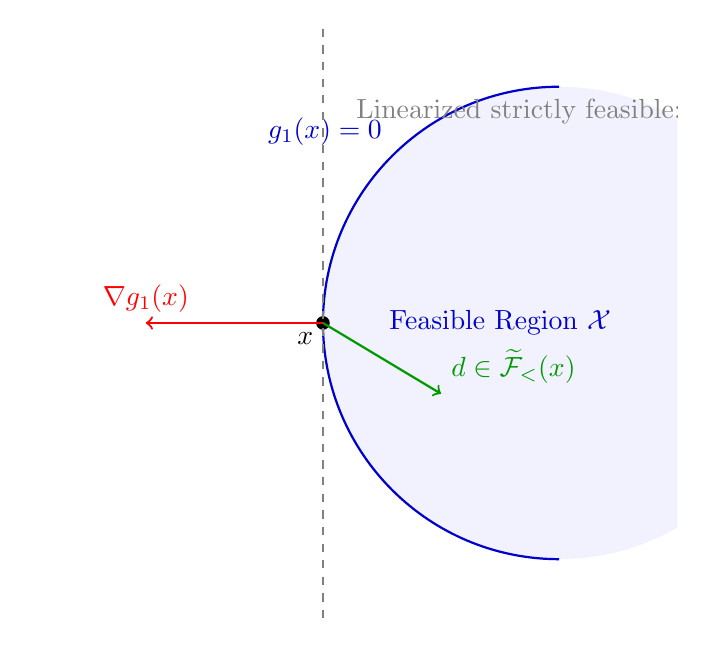
\begin{tikzpicture}[scale=1.5]
        % Clip region to keep diagram localized
        \clip (-2.5,-2.5) rectangle (3, 2.5);
        
        % The feasible region g(x) <= 0 (Circle centered at (2,0) with radius 2)
        \fill[blue!5] (2,0) circle (2);
        \draw[thick, blue!80!black] (0,0) arc (180:90:2) node[pos=0.5, above left] {$g_1(x)=0$};
        \draw[thick, blue!80!black] (0,0) arc (180:270:2);
        \node[blue!80!black] at (1.5, 0) {Feasible Region $\mathcal{X}$};
        
        % Point x (origin)
        \filldraw[black] (0,0) circle (1.5pt) node[anchor=north east] {$x$};
        
        % Gradient vector (Points outward, opposite to circle center)
        \draw[->, thick, red] (0,0) -- (-1.5, 0) node[above] {$\nabla g_1(x)$};
        
        % Tangent line (linearized constraint boundary)
        \draw[dashed, thick, gray] (0,-2.5) -- (0,2.5);
        \node[gray] at (0.2, 1.8) [anchor=west] {Linearized strictly feasible: $\nabla g_1(x)^\top d < 0$};
        
        % A direction d pointing inwards
        \draw[->, thick, green!60!black] (0,0) -- (1, -0.6) node[anchor=south west] {$d \in \widetilde{\mathcal{F}}_{<}(x)$};
        
    \end{tikzpicture}
    \caption{At point $x$, the gradient $\nabla g_1(x)$ points outwards (the direction of maximum objective increase). The condition $\nabla g_1(x)^\top d < 0$ defines the strict linearized feasible cone (the entire open half-space to the right of the dashed tangent line). As illustrated, any strictly linearized direction $d$ inevitably falls inside the actual curved feasible set $\mathcal{X}$ after taking a sufficiently small step $\alpha$.}
    \label{fig:feasible_cone}
\end{figure}

\begin{remark}
  A crucial consequence of $\widetilde{\mathcal{F}}_{<}(x) \subseteq \mathcal{F}(x)$ relates back to the optimality condition. If a point $x^*$ is a local minimum, Theorem~\ref{thm:local_min_dir} states $\mathcal{D}(x^*) \cap \mathcal{F}(x^*) = \emptyset$. Since the strict linearized cone is a subset of the actual feasible cone, this naturally implies:
  \[
    \widetilde{\mathcal{F}}_{<}(x^*) \cap \mathcal{D}(x^*) = \emptyset.
  \]
  This forms the foundation for algebraically identifying local minima by inspecting gradient arrays.
\end{remark}

% =====================================================================
\section{Necessity versus Sufficiency of the Characterization}
% =====================================================================

The condition $\widetilde{\mathcal{F}}_{<}(x^*) \cap \mathcal{D}(x^*) = \emptyset$ derived previously is a \textbf{necessary} condition for local optimality, but it is \textbf{not sufficient}. This means that finding a point $x^*$ that satisfies this condition does not guarantee that $x^*$ is actually a local minimum. To illustrate this and highlight the reliance on the functional form of the constraints, we consider two examples.

\begin{example}[A Point Satisfying the Necessary Condition that is NOT a Local Minimum]
  Consider the optimization problem:
  \begin{align*}
    \min_{x \in \mathbb{R}^2} \quad & x_1^2 + x_2^2 \\
    \text{subject to} \quad & h_1(x) = (x_1 + x_2 - 1)^3 \leq 0, \\
    & x_1 \geq 0, \quad x_2 \geq 0.
  \end{align*}
  Geometrically, the feasible region is the solid triangle defined by $x_1+x_2 \leq 1$ in the first quadrant. The objective represents the squared distance from the origin. Clearly, the true global minimum is at the origin $(0,0)$.
  
  Consider any point $x_A = (a,b)$ on the boundary line segment where $a+b=1$ (with $a > 0, b > 0$). At this point, the active constraint is $h_1(x)$. Let us compute the gradient of $h_1$ at $x_A$:
  \[
    \nabla h_1(x) = \begin{bmatrix} 3(x_1 + x_2 - 1)^2 \\ 3(x_1 + x_2 - 1)^2 \end{bmatrix} \implies \nabla h_1(x_A) = \begin{bmatrix} 0 \\ 0 \end{bmatrix}.
  \]
  The strictly linearized feasible cone at $x_A$ is defined by:
  \[
    \widetilde{\mathcal{F}}_{<}(x_A) = \{ d \in \mathbb{R}^2 : \nabla h_1(x_A)^\top d < 0 \} = \{ d \in \mathbb{R}^2 : \mathbf{0}^\top d < 0 \} = \emptyset.
  \]
  Since $\widetilde{\mathcal{F}}_{<}(x_A)$ is empty, its intersection with the descent cone $\mathcal{D}(x_A)$ is trivially empty:
  \[
    \widetilde{\mathcal{F}}_{<}(x_A) \cap \mathcal{D}(x_A) = \emptyset.
  \]
  Thus, $x_A$ perfectly satisfies the necessary condition for a local minimum. Yet, we know $x_A$ is emphatically \emph{not} a local minimum (from $x_A$, we can move straight down inside the triangle to decrease the objective). The failure here is that $\nabla h_1(x_A) = 0$ provides no local first-order geometric information about the boundary.
\end{example}

\begin{figure}[H]
    \centering
    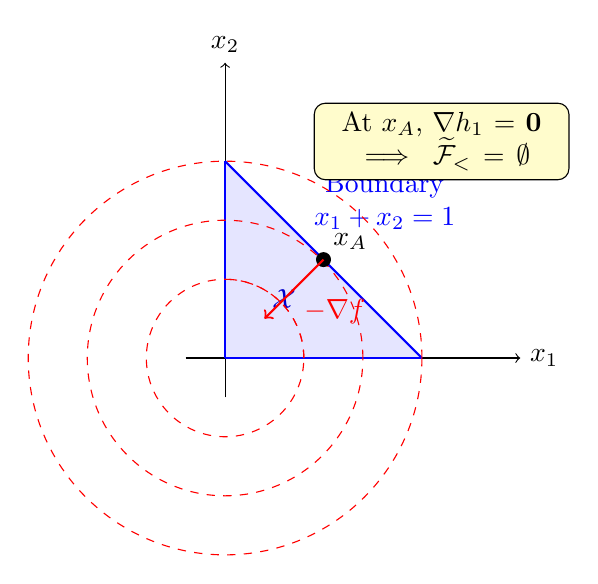
\begin{tikzpicture}[scale=2.5]
        % Axes
        \draw[->] (-0.2,0) -- (1.5,0) node[right] {$x_1$};
        \draw[->] (0,-0.2) -- (0,1.5) node[above] {$x_2$};
        
        % Feasible region
        \fill[blue!10] (0,0) -- (1,0) -- (0,1) -- cycle;
        \draw[thick, blue] (1,0) -- (0,1) node[pos=0.6, above right, align=center] {Boundary\\$x_1+x_2 = 1$};
        \draw[thick, blue] (0,0) -- (1,0);
        \draw[thick, blue] (0,0) -- (0,1);
        \node[blue!80!black] at (0.3, 0.3) {$\mathcal{X}$};
        
        % Level curves of x1^2 + x2^2
        \draw[dashed, red] (0,0) ++(45:0.4) arc (45:90:0.4);
        \draw[dashed, red] (0,0) ++(0:0.4) arc (0:45:0.4);
        \draw[dashed, red] (0,0) circle (0.4);
        \draw[dashed, red] (0,0) circle (0.7);
        \draw[dashed, red] (0,0) circle (1.0);
        
        % Point x_A
        \filldraw[black] (0.5,0.5) circle (1pt) node[anchor=south west] {$x_A$};
        
        % Gradient of h1
        \node[draw, fill=yellow!20, text width=3cm, align=center, rounded corners] at (1.1, 1.1) {At $x_A$, $\nabla h_1 = \mathbf{0}$ \\ $\implies \widetilde{\mathcal{F}}_{<} = \emptyset$};
        
        % Descent vector for objective
        \draw[->, thick, red] (0.5,0.5) -- (0.2,0.2) node[pos=0.5, anchor=north west] {$-\nabla f$};
    \end{tikzpicture}
    \caption{Visualizing Example 1: The point $x_A$ satisfies the necessary optimality conditions because the active constraint's gradient vanishes. However, the objective can clearly decrease by moving towards the origin within $\mathcal{X}$, proving the condition is not sufficient.}
    \label{fig:ex_cubic}
\end{figure}

\begin{example}[A Point Failing the Necessary Condition Appropriately]
  Let us slightly modify the previous problem by replacing the cubic constraint with a linear one representing the \emph{exact same geometric feasible set}:
  \begin{align*}
    \min_{x \in \mathbb{R}^2} \quad & x_1^2 + x_2^2 \\
    \text{subject to} \quad & h_1(x) = (x_1 + x_2 - 1) \leq 0, \\
    & x_1 \geq 0, \quad x_2 \geq 0.
  \end{align*}
  Consider the same point $x_A = (a,b)$ with $a+b=1$. Now, the gradient of the active constraint is:
  \[
    \nabla h_1(x_A) = \begin{bmatrix} 1 \\ 1 \end{bmatrix}.
  \]
  The strictly linearized feasible cone is no longer empty:
  \[
    \widetilde{\mathcal{F}}_{<}(x_A) = \left\{ d \in \mathbb{R}^2 : d_1 + d_2 < 0 \right\} \neq \emptyset.
  \]
  We can compute the descent cone for the objective. The gradient of $f(x)=x_1^2+x_2^2$ is $\nabla f(x_A) = [2a, 2b]^\top$. So the descent cone is:
  \[
    \mathcal{D}(x_A) = \left\{ d \in \mathbb{R}^2 : 2a d_1 + 2b d_2 < 0 \right\}.
  \]
  It is trivial to find a direction $d$ that belongs to both sets (e.g., $d = [-a, -b]^\top$, which is moving straight towards the origin, yielding $-a-b = -1 < 0$ and $-2a^2-2b^2 < 0$). Thus,
  \[
    \widetilde{\mathcal{F}}_{<}(x_A) \cap \mathcal{D}(x_A) \neq \emptyset.
  \]
  This correctly flags that $x_A$ is \emph{not} a local minimum, showing how deeply the necessary condition relies on a non-degenerate algebraic representation (non-vanishing gradients) of the constraints.
\end{example}

\subsection{The Limitation Handling Equality Constraints}

The necessary condition $\widetilde{\mathcal{F}}_{<}(x^*) \cap \mathcal{D}(x^*) = \emptyset$ is immensely powerful for inequality constraints $h_j(x) \leq 0$. However, it completely breaks down when applied naively to \textbf{equality constraints}. Let us examine why this happens.

\begin{example}[Equality Constraints Lead to Trivial Linearized Cones]
  Suppose we have an equality constraint $x_1 + x_2 - 1 = 0$. A standard technique to handle an equality constraint is to split it into two opposing inequality constraints:
  \begin{align*}
    h_1(x) &= (x_1 + x_2 - 1) \leq 0 \\
    h_2(x) &= -(x_1 + x_2 - 1) \leq 0
  \end{align*}
  If a point $x_A$ is feasible (meaning it lies on the line $x_1 + x_2 - 1 = 0$), then both $h_1$ and $h_2$ are tightly active at $0$.
  Computing the gradients yields:
  \[
    \nabla h_1(x_A) = \begin{bmatrix} 1 \\ 1 \end{bmatrix}, \quad \nabla h_2(x_A) = \begin{bmatrix} -1 \\ -1 \end{bmatrix}.
  \]
  To find the strictly linearized feasible cone, a direction $d$ must simultaneously satisfy both strict inner product conditions:
  \begin{align*}
    \nabla h_1(x_A)^\top d < 0 &\implies d_1 + d_2 < 0 \\
    \nabla h_2(x_A)^\top d < 0 &\implies -(d_1 + d_2) < 0 \implies d_1 + d_2 > 0
  \end{align*}
  It is mathematically impossible for $d_1 + d_2$ to be strictly less than $0$ and strictly greater than $0$ at the same time. Therefore,
  \[
    \widetilde{\mathcal{F}}_{<}(x_A) = \emptyset.
  \]
  Because the set is empty, $\widetilde{\mathcal{F}}_{<}(x_A) \cap \mathcal{D}(x_A) = \emptyset$ will hold trivially for \emph{any} point on the feasibility line, turning the condition into a tautology regardless of whether the point is a local minimum or not.
\end{example}

\begin{figure}[H]
    \centering
    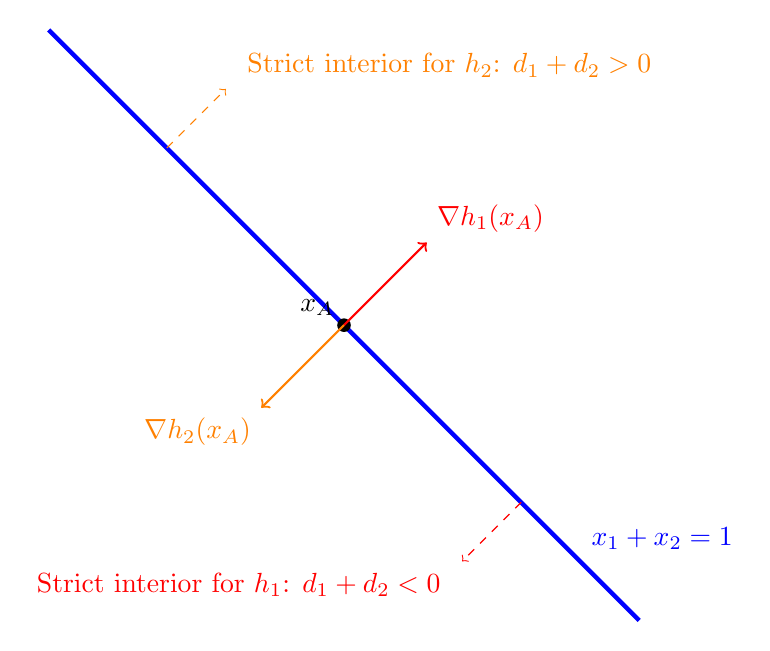
\begin{tikzpicture}[scale=1.5]
        % The line x1 + x2 = 1
        \draw[ultra thick, blue] (-2, 3) -- (3, -2) node[pos=0.9, above right] {$x_1+x_2=1$};
        
        % Point x_A
        \filldraw[black] (0.5,0.5) circle (1.5pt) node[above left] {$x_A$};
        
        % Gradient vectors
        \draw[->, thick, red] (0.5,0.5) -- (1.2,1.2) node[above right] {$\nabla h_1(x_A)$};
        \draw[->, thick, orange] (0.5,0.5) -- (-0.2,-0.2) node[below left] {$\nabla h_2(x_A)$};
        
        % Half plane arrows
        \draw[->, dashed, red] (2, -1) -- (1.5, -1.5);
        \draw[->, dashed, orange] (-1, 2) -- (-0.5, 2.5);
        
        \node[align=right, red, anchor=east] at (1.4, -1.7) {Strict interior for $h_1$: $d_1+d_2 < 0$};
        \node[align=left, orange, anchor=west] at (-0.4, 2.7) {Strict interior for $h_2$: $d_1+d_2 > 0$};
    \end{tikzpicture}
    \caption{Visualizing Example 3: An equality constraint modelled as two inequalities. The strict feasible directions for $h_1$ point into the open half-space below the line, and those for $h_2$ point strictly above it. The intersection of these two open half-spaces is empty, trivially leading to $\widetilde{\mathcal{F}}_{<} = \emptyset$.}
    \label{fig:ex_equality}
\end{figure}

\begin{tcolorbox}[colframe=red!70!black, colback=red!5!white, title=Important Limitation]
  The strict interior cone characterization $\widetilde{\mathcal{F}}_{<}(x^*) \cap \mathcal{D}(x^*) = \emptyset$ is \textbf{strictly applicable only for inequality constraints}. For systems containing equality constraints, we must rely on closed tangent cones or directly use the KKT gradient matrix stationarity conditions directly.
\end{tcolorbox}

% =====================================================================
\section{Matrix Representation of the Local Minimum Characterization}
% =====================================================================

Let $x^* \in \mathcal{X}$ and let the active constraint index set be $\mathcal{A}(x^*) = \{i_1, i_2, \ldots, i_k\}$ for some $k \leq m$. Define the \textbf{active constraint gradient matrix}:

\[
  G =
  \begin{bmatrix}
    \nabla g_{i_1}(x^*)^\top \\
    \nabla g_{i_2}(x^*)^\top \\
    \vdots \\
    \nabla g_{i_k}(x^*)^\top
  \end{bmatrix} \in \mathbb{R}^{k \times n}.
\]

The linearized feasible cone and descent set become:
\begin{align*}
  \widetilde{\mathcal{F}}(x^*) &= \{d \in \mathbb{R}^n : Gd \leq 0\}, \\
  \mathcal{D}(x^*)             &= \{d \in \mathbb{R}^n : \nabla f(x^*)^\top d < 0\}.
\end{align*}

\textbf{Necessary condition in matrix form.} The condition $\mathcal{D}(x^*) \cap \widetilde{\mathcal{F}}(x^*) = \emptyset$ states:

\[
  \boxed{\text{There is no } d \in \mathbb{R}^n \text{ such that } \nabla f(x^*)^\top d < 0 \text{ and } Gd \leq 0.}
\]

By Farkas' Lemma (Theorem~\ref{thm:farkas_opt}), this is equivalent to the existence of a vector $\lambda \in \mathbb{R}^k$, $\lambda \geq 0$, such that:
\[
  \nabla f(x^*) + G^\top \lambda = 0 \quad \Longleftrightarrow \quad \nabla f(x^*) = -\sum_{j=1}^{k} \lambda_{i_j} \nabla g_{i_j}(x^*).
\]

Extending to all constraints with $\lambda_i = 0$ for $i \notin \mathcal{A}(x^*)$, we get the \textbf{KKT stationarity condition}:
\[
  \nabla f(x^*) + \sum_{i=1}^{m} \lambda_i \nabla g_i(x^*) = 0, \qquad \lambda_i \geq 0, \quad \lambda_i g_i(x^*) = 0 \;\; \forall\, i.
\]

The last condition $\lambda_i g_i(x^*) = 0$ (complementary slackness) follows because $\lambda_i = 0$ for all inactive constraints (by construction) and $g_i(x^*) = 0$ for all active ones.

\textbf{Summary in compact matrix form.}

\begin{tcolorbox}[colback=blue!5, colframe=blue!60!black, title=Local Minimum Characterization (Matrix Form)]
$x^*$ is a local minimum of $\min f(x)$ s.t.\ $g_i(x) \leq 0$ only if there exist $\lambda \in \mathbb{R}^m$, $\lambda \geq 0$, such that:
\begin{align*}
  \nabla f(x^*) + G^\top \lambda_{\mathcal{A}} &= 0 \quad \text{(Stationarity)}, \\
  G x^* &= 0 \quad \text{(Active constraint at } x^*\text{)}, \\
  \lambda_{\mathcal{A}} &\geq 0 \quad \text{(Non-negativity of multipliers)},
\end{align*}
where $G \in \mathbb{R}^{|\mathcal{A}(x^*)| \times n}$ is the active constraint gradient matrix and $\lambda_{\mathcal{A}}$ are the associated multipliers.
\end{tcolorbox}

% =====================================================================
\section{Farkas' Lemma and Its Translation to Optimality}
\label{sec:farkas}
% =====================================================================

The transition from the geometric condition $\widetilde{\mathcal{F}}_{<}(x^*) \cap \mathcal{D}(x^*) = \emptyset$ (derived in previous sections) to the algebraic KKT stationarity condition relies fundamentally on a theorem of alternatives known as Farkas' Lemma.

\begin{theorem}[Farkas' Lemma]
  Let $A \in \mathbb{R}^{m \times n}$ be a given matrix, and $c \in \mathbb{R}^n$ a given vector. Then exactly one of the following two systems has a solution:
  \begin{enumerate}
    \item System 1: $Ax \leq 0 \quad \text{and} \quad c^\top x < 0$ for some $x \in \mathbb{R}^n$.
    \item System 2: $A^\top y = c \quad \text{and} \quad y \geq 0$ for some $y \in \mathbb{R}^m$.
  \end{enumerate}
\end{theorem}

Geometrically, Farkas' lemma states that either the vector $c$ lies within the convex cone generated by the rows of $A$ (System 2), or there exists a hyperplane passing through the origin that strictly separates $c$ from that cone (System 1).

\begin{figure}[H]
    \centering
    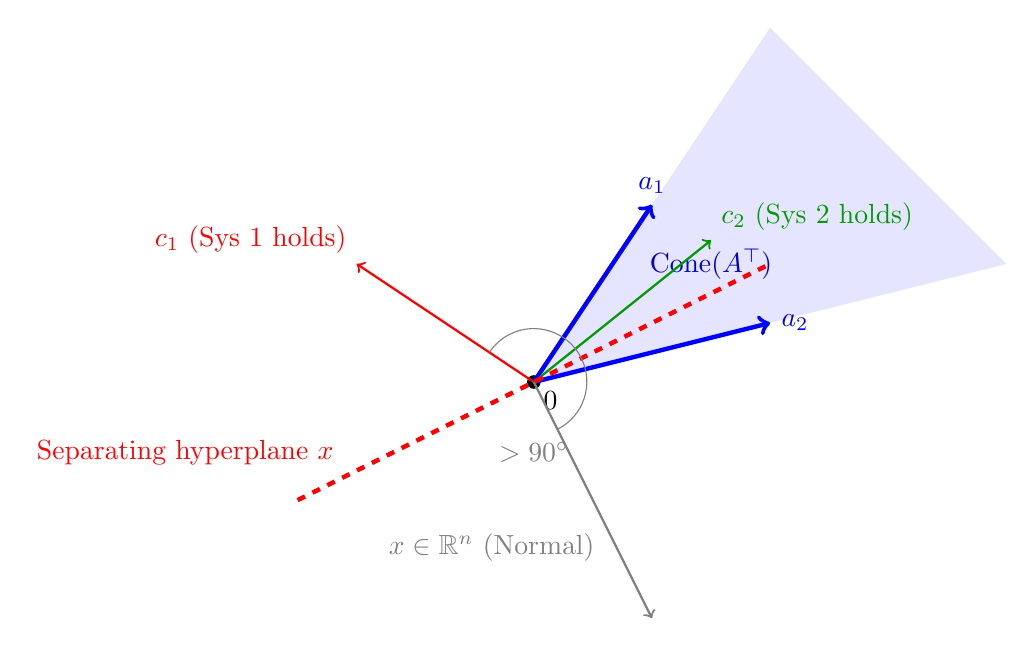
\begin{tikzpicture}[scale=1.5]
        % Origin
        \filldraw[black] (0,0) circle (1.5pt) node[below right] {$0$};
        
        % Rows of A (Generators of the cone)
        \draw[->, ultra thick, blue] (0,0) -- (1, 1.5) node[above] {$a_1$};
        \draw[->, ultra thick, blue] (0,0) -- (2, 0.5) node[right] {$a_2$};
        
        % The shaded cone
        \fill[blue, opacity=0.1] (0,0) -- (2,3) -- (4,1) -- cycle;
        \node[blue!80!black] at (1.5, 1) {Cone($A^\top$)};
        
        % Case 1: c is inside the cone
        \draw[->, thick, green!60!black] (0,0) -- (1.5, 1.2) node[above right] {$c_2$ (Sys 2 holds)};
        
        % Case 2: c is outside the cone
        \draw[->, thick, red] (0,0) -- (-1.5, 1) node[above left] {$c_1$ (Sys 1 holds)};
        
        % Separating hyperplane for c1
        \draw[dashed, ultra thick, red] (-2, -1) -- (2, 1) node[pos=0.1, above left] {Separating hyperplane $x$};
        
        % Normal x (pointing downwards-right, orthogonal to the red line y = 1/2 x)
        \draw[->, thick, gray] (0,0) -- (1, -2) node[pos=0.6, below left] {$x \in \mathbb{R}^n$ (Normal)};
        
        % Show inner angle
        \draw[gray] (0.2, -0.4) arc (-63.4:146.3:0.45);
        \node[gray] at (0,-0.6) {$>90^\circ$};
    \end{tikzpicture}
    \caption{Visualizing Farkas' Lemma. For a vector $c_2$ situated inside the cone spanned by the rows of $A$ (i.e. $a_1, a_2$), it can be represented as a non-negative linear combination $y_1 a_1 + y_2 a_2$ (System 2). Conversely, if $c_1$ is strictly outside the cone, we can find a strictly separating hyperplane. The normal vector to this hyperplane, $x$, acts as a direction making an obtuse angle with $c_1$ ($c_1^\top x < 0$) and obtuse/right angles with the cone generators ($a_i^\top x \leq 0 \implies Ax \leq 0$) (System 1).}
    \label{fig:farkas}
\end{figure}

\begin{corollary}[Optimality via Farkas' Lemma]
  \label{thm:farkas_opt}
  Let us apply Farkas' Lemma to our derived necessary condition $\widetilde{\mathcal{F}}_{<}(x^*) \cap \mathcal{D}(x^*) = \emptyset$.
  
  Recall this geometric condition means there exists no direction $d \in \mathbb{R}^n$ such that:
  \[
    Gd \leq 0 \quad \text{and} \quad \nabla f(x^*)^\top d < 0
  \]
  where $G \in \mathbb{R}^{k \times n}$ is the matrix whose rows are the gradients of the active constraints $\nabla g_{i_j}(x^*)^\top$.
  
  Identifying our variables with Farkas' Lemma:
  \begin{itemize}
    \item $x \longleftrightarrow d$ (The search direction)
    \item $A \longleftrightarrow G$ (The active constraint normal matrix)
    \item $c \longleftrightarrow \nabla f(x^*)$ (The objective gradient)
  \end{itemize}
  Since we established that System 1 has \emph{NO mathematical solution} at a strict local minimum point $x^*$, it logically necessitates that System 2 \emph{MUST have a solution}.
  
  Therefore, there exists a vector of non-negative multipliers $\lambda_{\mathcal{A}} \geq 0$ (corresponding to the active constraints) such that:
  \[
    G^\top \lambda_{\mathcal{A}} = -\nabla f(x^*) \implies \nabla f(x^*) + G^\top \lambda_{\mathcal{A}} = \mathbf{0} \implies \nabla f(x^*) + \sum_{j=1}^{k} \lambda_{i_j} \nabla g_{i_j}(x^*) = \mathbf{0}.
  \]
  This perfectly bridges the gap, translating the conceptual lack of geometric descent directions into the clean algebraic KKT stationarity equations that we solve in practice.
\end{corollary}

\bigskip

\begin{thebibliography}{9}
\end{thebibliography}

\end{document}